\chapter{Architecture Patterns \\
\small{\textit{-- ZKD, KRV, CL, \& ZZ}}
\index{Architecture Patterns} 
\index{Chapter!Architecture Patterns}
\label{Chapter::Architecture Patterns}}

\section{Search Engine}
Assuming we have a very large dataset of shoes with various brands, styles, colors and sizes like Zappos \cite{zappos} does, we need to figure out which architectural pattern should be applied for basic search engine capability of our enormous dataset.

\subsection{Pipe and Filter Pattern}
For a basic search engine to handle a large dataset of shoes (brands, styles, colors, sizes), the Pipe and Filter Pattern is an excellent fit.

\subsection{Why Pipe and Filter?}
\begin{itemize}[leftmargin=*, label={\textbullet}]
    \item \textbf{Context}: You need to transform and process streams of data (search queries and shoe datasets) in a modular, scalable way.
    
    \item \textbf{Problem}: The system needs to be divided into reusable, loosely coupled components that can be flexibly combined and scaled.
    
    \item \textbf{Solution}: Pipe and Filter allows for data to be processed in filters, with each filter handling a specific part of the search query---like filtering by brand, style, color, or size---and outputting refined results down the line.
\end{itemize}

\begin{figure}[h]
    \centering
    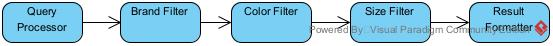
\includegraphics[scale=0.7]{Book-SSW565/jpg/ArchitecturePatterns/Pipe and Filter.jpg}
    \caption{\label{Figure::Pipe and Filter}Pipe and Filter}
\end{figure}

\subsection{Component and Connector Pattern}
To support user access to the search engine, the Client-Server Pattern (from the Component and Connector patterns) is a great choice. It enables the system to support multiple users searching for shoes concurrently, with the server side managing and processing requests. Client-Server to provide user access and support distributed users interacting with the system.

\begin{figure}[h]
    \centering
    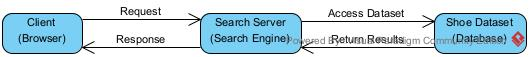
\includegraphics[scale=0.7]{Book-SSW565/jpg/ArchitecturePatterns/Component and Connector Pattern.jpg}
    \caption{\label{Figure::Component and Connector Pattern}Component and Connector Pattern}
\end{figure}

\section{Model View Controller}
\begin{lstlisting}[caption=model.py]
# model.py
class User:
    def __init__(self, name, age):
        self.name = name
        self.age = age

class UserModel:
    def __init__(self):
        self.users = []  # Simulating a database

    def add_user(self, name, age):
        user = User(name, age)
        self.users.append(user)

    def get_users(self):
        return self.users
\end{lstlisting}
\begin{lstlisting}[caption=view.py]
# view.py
class UserView:
    def __init__(self):
          pass # good for a breakpoint

    @staticmethod
    def show_users(users):
        print("\nUser List:")
        for user in users:
            print(f"Name: {user.name}, Age: {user.age}")

    @staticmethod
    def show_message(message):
        print(message)
\end{lstlisting}

\begin{lstlisting}[caption=controller.py]
# controller.py
from model import UserModel
from view import UserView


class UserController:
    def __init__(self):
        self.model = UserModel()
        self.view = UserView()

    def add_user(self, name, age):
        self.model.add_user(name, age)
        self.view.show_message(f"User '{name}' added successfully!")

    def display_users(self):
        users = self.model.get_users()
        self.view.show_users(users)


# Run the MVC
if __name__ == "__main__":
    controller = UserController()

    controller.add_user("Alice", 25)
    controller.add_user("Bob", 30)

    controller.display_users()

\end{lstlisting}

\subsection{Class Diagram}
\begin{figure}[H]
    \centering
    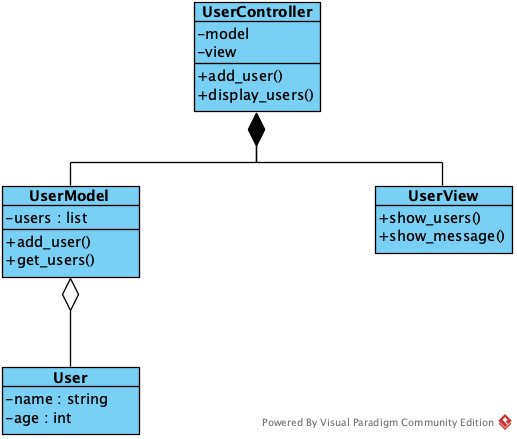
\includegraphics[scale=0.8]{Book-SSW565/jpg/ArchitecturePatterns/MVC Class Diagram.png}
    \caption{\label{Figure::MVC Class Diagram}MVC Class Diagram}
\end{figure}

\subsection{Object Diagram}
\begin{figure}[H]
    \centering
    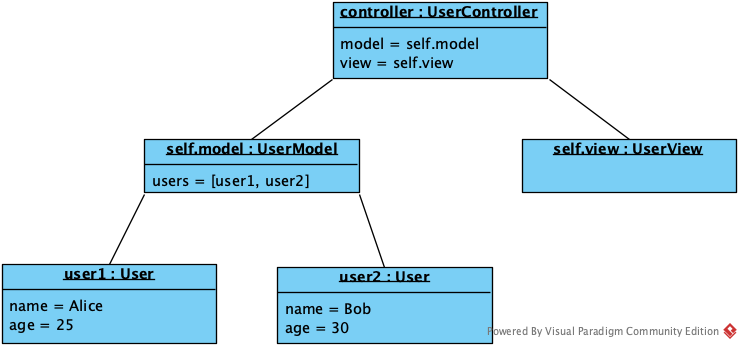
\includegraphics[scale=0.7]{Book-SSW565/jpg/ArchitecturePatterns/ScenarioObjectDiagram.png}
    \caption{\label{Figure::MVC Object Diagram}MVC Object Diagram}
\end{figure}

\subsection{Sequence Diagram}
\begin{figure}[H]
    \centering
    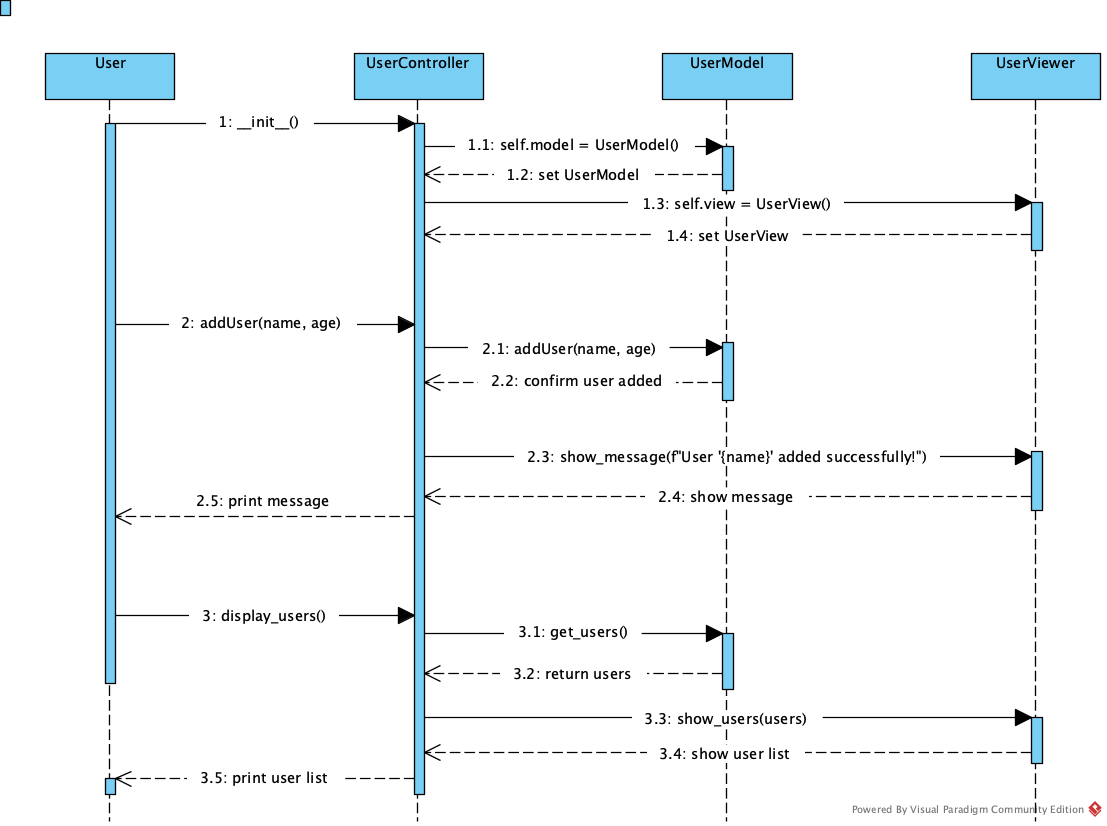
\includegraphics[scale=0.7]{Book-SSW565/jpg/ArchitecturePatterns/MVCSequenceDiagram.png}
    \caption{\label{Figure::MVC Sequence Diagram}MVC Sequence Diagram}
\end{figure}


\section{In-Class Exercise: Redesigned Oscilloscope}
Redesigning the Oscilloscope using the "MVC" for the user interface and "Pipe and Filter" for the signal processing part. Assuming that the two filters we have are: scpScale (to scale the signal) and scpOffset to offset the signal.

\subsection{MVC and Pipe-Filter Patterns}
\begin{enumerate}
  \item  \textbf{Model-View-Controller (MVC) for Oscilloscope UI}
  \newline \textbf{Description:}
    \begin{itemize}
        \item  \textbf{Model:}
        \newline Represents Oscilloscope data.(waveforms, voltage readers, etc.)
        \item \textbf{View:}
        \newline Handles display functions.
        \item \textbf{Controller:}
        \newline Manages user interaction and updates the model.
    \end{itemize}
  \item \textbf{Pipe and Filter Pattern for Signal Processing}
  \newline \textbf{Description:}
  \newline The Pipe and Filter pattern is used to process oscilloscope signals through a sequence and parallel of operations.
  \begin{itemize}
      \item \textbf{Filters:}
      \newline Modify signal data (scaling, offset adjustments).
      \item \textbf{Pipes:}
      \newline Pass the transformed signal between filters. or Perform parallel work by filters on the raw waveform data.
  \end{itemize}
  In the oscilloscope redesign using the Pipe and Filter pattern, we can incorporate parallel processing where applicable.
  \newline \textbf{Parallel Approach:}
  \begin{itemize}
      \item We consider scpScale and scpOffset are not depend on each other's results, they can be processed simultaneously in parallel.
      \item The raw input signal is split and sent to both filters at the same time.
      \item After both filters finish processing, the results are merged back before passing to the display.
  \end{itemize}
\end{enumerate}

\subsection{Class Diagram}
\subsection{Object Diagram}
\subsection{Sequence Diagram}